\documentclass[11pt,a4paper]{article}

% ══════════════════════════════════════════════════════════════
% PACKAGES
% ══════════════════════════════════════════════════════════════
\usepackage[margin=2.2cm,top=2.5cm,bottom=2.5cm]{geometry}
\usepackage{amsmath,amssymb,amsfonts}
\usepackage{graphicx}
\usepackage[dvipsnames,svgnames,x11names]{xcolor}
\usepackage{tikz}
\usetikzlibrary{shapes,arrows.meta,positioning,calc,decorations.pathreplacing,shadows,fit}
\usepackage{booktabs}
\usepackage{tabularx}
\usepackage{longtable}
\usepackage{fancyhdr}
\usepackage{hyperref}
\usepackage{enumitem}
\usepackage{multicol}
\usepackage{tcolorbox}
\tcbuselibrary{skins,breakable}
\usepackage{fontenc}
%\usepackage{microtype} % disabled - font expansion issue
\usepackage{titlesec}
\usepackage{float}
\usepackage{wrapfig}
\usepackage{setspace}
\usepackage{parskip}

% ══════════════════════════════════════════════════════════════
% COLORS
% ══════════════════════════════════════════════════════════════
\definecolor{qnkpurple}{HTML}{7C3AED}
\definecolor{qnkblue}{HTML}{3B82F6}
\definecolor{qnkcyan}{HTML}{06B6D4}
\definecolor{qnkgreen}{HTML}{10B981}
\definecolor{qnkamber}{HTML}{F59E0B}
\definecolor{qnkred}{HTML}{EF4444}
\definecolor{qnkdark}{HTML}{0F172A}
\definecolor{qnkslate}{HTML}{334155}
\definecolor{qnkgold}{HTML}{D4AF37}
\definecolor{sectioncolor}{HTML}{5B21B6}
\definecolor{boxbg}{HTML}{F5F3FF}
\definecolor{keyboxbg}{HTML}{EFF6FF}

% ══════════════════════════════════════════════════════════════
% STYLING
% ══════════════════════════════════════════════════════════════
\hypersetup{
    colorlinks=true,
    linkcolor=qnkpurple,
    urlcolor=qnkblue,
    citecolor=qnkpurple,
    pdfauthor={Q-NarwhalKnight Foundation},
    pdftitle={Q-NarwhalKnight Investor Pitch},
}

\pagestyle{fancy}
\fancyhf{}
\fancyhead[L]{\small\textcolor{qnkslate}{Q-NarwhalKnight --- Confidential Investor Materials}}
\fancyhead[R]{\small\textcolor{qnkslate}{February 2026}}
\fancyfoot[C]{\small\textcolor{qnkslate}{\thepage}}
\renewcommand{\headrulewidth}{0.4pt}

\titleformat{\section}{\Large\bfseries\color{sectioncolor}}{}{0em}{}[\vspace{-0.5em}\textcolor{qnkpurple}{\rule{\textwidth}{1.5pt}}]
\titleformat{\subsection}{\large\bfseries\color{qnkslate}}{}{0em}{}

% Custom boxes
\newtcolorbox{keyinsight}[1][]{
    enhanced,
    colback=keyboxbg,
    colframe=qnkblue,
    boxrule=1pt,
    arc=4pt,
    left=10pt, right=10pt, top=8pt, bottom=8pt,
    fonttitle=\bfseries\color{qnkblue},
    title={#1},
    shadow={1mm}{-1mm}{0mm}{black!15}
}

\newtcolorbox{highlight}[1][]{
    enhanced,
    colback=boxbg,
    colframe=qnkpurple,
    boxrule=1pt,
    arc=4pt,
    left=10pt, right=10pt, top=8pt, bottom=8pt,
    fonttitle=\bfseries\color{qnkpurple},
    title={#1},
    shadow={1mm}{-1mm}{0mm}{black!15}
}

\newtcolorbox{warningbox}[1][]{
    enhanced,
    colback=red!5,
    colframe=qnkred,
    boxrule=1pt,
    arc=4pt,
    left=10pt, right=10pt, top=8pt, bottom=8pt,
    fonttitle=\bfseries\color{qnkred},
    title={#1}
}

\newtcolorbox{successbox}[1][]{
    enhanced,
    colback=green!5,
    colframe=qnkgreen,
    boxrule=1pt,
    arc=4pt,
    left=10pt, right=10pt, top=8pt, bottom=8pt,
    fonttitle=\bfseries\color{qnkgreen!70!black},
    title={#1}
}

% ══════════════════════════════════════════════════════════════
% DOCUMENT
% ══════════════════════════════════════════════════════════════
\begin{document}

% ──────────────────────────────────────────────────────────────
% TITLE PAGE
% ──────────────────────────────────────────────────────────────
\thispagestyle{empty}
\begin{center}
\vspace*{2cm}

% Logo area
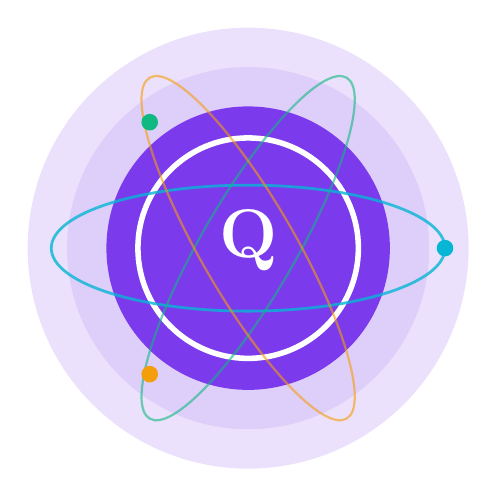
\begin{tikzpicture}
    % Outer glow
    \fill[qnkpurple!15] (0,0) circle (2.8cm);
    \fill[qnkpurple!25] (0,0) circle (2.3cm);
    % Main circle
    \fill[qnkpurple] (0,0) circle (1.8cm);
    % Inner ring
    \draw[white, line width=2pt] (0,0) circle (1.4cm);
    % Q letter
    \node[white, font=\fontsize{48}{48}\selectfont\bfseries] at (0,0.1) {Q};
    % Quantum orbit lines
    \draw[qnkcyan, line width=1pt, opacity=0.8] (0,0) ellipse (2.5cm and 0.8cm);
    \draw[qnkgreen, line width=0.8pt, opacity=0.6, rotate=60] (0,0) ellipse (2.5cm and 0.6cm);
    \draw[qnkamber, line width=0.8pt, opacity=0.6, rotate=-60] (0,0) ellipse (2.5cm and 0.6cm);
    % Electron dots
    \fill[qnkcyan] (2.5,0) circle (3pt);
    \fill[qnkgreen] (-1.25,1.6) circle (3pt);
    \fill[qnkamber] (-1.25,-1.6) circle (3pt);
\end{tikzpicture}

\vspace{1.5cm}

{\fontsize{36}{42}\selectfont\bfseries\textcolor{qnkdark}{Q-NarwhalKnight}}

\vspace{0.3cm}

{\Large\textcolor{qnkslate}{The Quantum-Ready Blockchain}}

\vspace{0.5cm}

{\large\textcolor{qnkpurple}{\textit{Where Physics Meets Finance}}}

\vspace{2cm}

\textcolor{qnkslate}{\rule{8cm}{0.5pt}}

\vspace{0.5cm}

{\large\textbf{Investor Pitch \& Technical Overview}}

\vspace{0.3cm}

{\textcolor{qnkslate}{February 2026 --- Confidential}}

\vspace{2cm}

\begin{tcolorbox}[
    enhanced,
    colback=qnkpurple!5,
    colframe=qnkpurple!50,
    boxrule=0.5pt,
    arc=8pt,
    width=12cm,
    center,
    fontupper=\centering
]
{\small\textcolor{qnkslate}{
\textbf{500,000+ lines of Rust} $\cdot$ \textbf{83 modular crates} $\cdot$ \textbf{4,000+ tests}\\[4pt]
\textbf{Live testnet} $\cdot$ \textbf{Post-quantum native} $\cdot$ \textbf{Decentralized AI}\\[4pt]
\textbf{Zero-knowledge privacy} $\cdot$ \textbf{Physics-grounded consensus}
}}
\end{tcolorbox}

\vfill

{\small\textcolor{qnkslate}{
\textbf{Website:} quillon.xyz \quad$\cdot$\quad \textbf{Testnet:} \url{https://quillon.xyz}
}}

\end{center}
\newpage

% ──────────────────────────────────────────────────────────────
% TABLE OF CONTENTS
% ──────────────────────────────────────────────────────────────
\tableofcontents
\newpage

% ══════════════════════════════════════════════════════════════
% SECTION 1: EXECUTIVE SUMMARY
% ══════════════════════════════════════════════════════════════
\section{Executive Summary}

Q-NarwhalKnight is a \textbf{production-ready, quantum-resistant Layer~1 blockchain} that unifies post-quantum cryptography, zero-knowledge privacy, decentralized artificial intelligence, and physics-inspired consensus under a single mathematical framework---the \textit{K-Parameter Master Equation}.

\begin{highlight}[The Thesis in One Sentence]
The quantum computing revolution will render every existing blockchain's cryptography obsolete within this decade; Q-NarwhalKnight is the \textbf{only} Layer~1 that has already completed the transition, shipping 500,000+ lines of production Rust code with native post-quantum security at every protocol layer.
\end{highlight}

\subsection{Key Metrics at a Glance}

\begin{center}
\begin{tabular}{@{}p{5.5cm}p{9cm}@{}}
\toprule
\textbf{Metric} & \textbf{Value} \\
\midrule
Consensus Protocol & DAG-Knight + Narwhal mempool + Bullshark finality \\
Throughput & 27,200+ TPS (theoretical), 2,800+ TPS (measured) \\
Finality & $<3$ seconds \\
Post-Quantum Signatures & Dilithium5 (NIST Level 5) + SQIsign (204 bytes) \\
Key Exchange & Kyber1024 (NIST Level 5, lattice-based) \\
Mining & SHA-3 + VDF (ASIC-resistant, consumer hardware) \\
Privacy & Ring sigs + Stealth + ZK-STARKs + Tor + Dandelion++ \\
AI & Mistral-7B distributed inference across validators \\
Codebase & 500,000+ LOC Rust across 83 crates \\
Test Suite & 4,000+ automated tests incl.\ mainnet safety \\
Total Supply & 21,000,000 QUG (hard cap) \\
\bottomrule
\end{tabular}
\end{center}

% ══════════════════════════════════════════════════════════════
% SECTION 2: THE PROBLEM
% ══════════════════════════════════════════════════════════════
\section{The Problem: An Existential Threat to Blockchain}

\subsection{The Quantum Apocalypse Is Not Hypothetical}

Every major blockchain---Bitcoin, Ethereum, Solana, Cardano---relies on \textbf{elliptic curve cryptography} (ECDSA, Ed25519) for transaction signing and \textbf{Diffie-Hellman} variants for key exchange. Peter Shor's quantum algorithm, published in 1994, can break both in polynomial time on a sufficiently large quantum computer.

This is not a distant threat:
\begin{itemize}[leftmargin=1.5em]
    \item \textbf{IBM Quantum Heron} (2024): 1,121 physical qubits with record-low error rates
    \item \textbf{Google Willow} (2024): Demonstrated quantum error correction below threshold
    \item \textbf{NIST FIPS 203/204/205} (2024): Finalized post-quantum algorithm standards---acknowledging the threat is real enough to standardize against
    \item \textbf{NSA CNSA 2.0} (2022): Mandates post-quantum algorithms for all classified systems by 2035
    \item \textbf{``Harvest Now, Decrypt Later''}: Nation-state adversaries are already storing encrypted blockchain traffic for future quantum decryption
\end{itemize}

\begin{warningbox}[The \$3 Trillion Risk]
The total cryptocurrency market capitalization exceeds \$3 trillion. \textbf{None} of the top 20 blockchains by market cap have implemented post-quantum cryptography at the consensus layer. Every transaction signed today with ECDSA will be forgeable by a sufficiently powerful quantum computer. The blockchain industry is sitting on an unhedged existential risk.
\end{warningbox}

\subsection{Four Compounding Failures}

Beyond quantum vulnerability, existing blockchains suffer from four interconnected failures:

\begin{enumerate}[leftmargin=1.5em]
    \item \textbf{Transparent Ledgers Destroy Privacy.} Bitcoin and Ethereum expose every transaction, sender, recipient, and amount on a public ledger. Chain analysis firms like Chainalysis can trace funds with 95\%+ accuracy. This is incompatible with financial privacy rights (GDPR Article 5, ECHR Article 8).

    \item \textbf{AI Centralization Creates Dependency.} As AI becomes essential for DeFi (risk assessment, market analysis, fraud detection), blockchains depend entirely on centralized APIs (OpenAI, Google). This creates single points of failure, data leakage, and censorship risk.

    \item \textbf{Classical BFT Has Fundamental Limits.} Traditional Byzantine Fault Tolerance requires $n \geq 3f + 1$ validators to tolerate $f$ Byzantine faults. This sets high infrastructure costs and limits decentralization.

    \item \textbf{Mining Centralization via ASICs.} Bitcoin's SHA-256 mining is dominated by ASIC manufacturers (Bitmain, MicroBT). Consumer hardware cannot compete, centralizing block production to a handful of industrial operations.
\end{enumerate}

\begin{keyinsight}[The Opportunity]
The first Layer~1 blockchain to solve quantum security \textit{with} privacy \textit{with} AI \textit{at scale} captures the next generation of institutional and sovereign adoption. This is not an incremental improvement---it is a paradigm shift.
\end{keyinsight}

% ══════════════════════════════════════════════════════════════
% SECTION 3: THE SOLUTION
% ══════════════════════════════════════════════════════════════
\section{The Solution: Q-NarwhalKnight}

Q-NarwhalKnight addresses all four failures simultaneously through five integrated pillars.

\subsection{Pillar 1: Quantum Security at Every Layer}

Post-quantum cryptography is not bolted on---it is \textbf{native} to every protocol layer:

\begin{center}
\begin{tabular}{@{}lll@{}}
\toprule
\textbf{Layer} & \textbf{Algorithm} & \textbf{Security Basis} \\
\midrule
Transaction signing & Dilithium5 & Module-LWE (NIST Level 5) \\
Certificate signing & SQIsign & Supersingular isogenies (204 bytes) \\
Key exchange & Kyber1024 & Module-LWE (NIST Level 5) \\
Symmetric encryption & AEGIS-256 & AES-based AEAD (2--5$\times$ faster) \\
VDF mining & Genus-2 VDF & Hyperelliptic curve time-locking \\
Ring signatures & Module-LWE & Lattice-based unlinkability \\
Threshold signing & FROST & Schnorr-based multi-party \\
Aggregate signatures & Lattice & 98\% bandwidth reduction \\
\bottomrule
\end{tabular}
\end{center}

\textbf{Why this matters:} A quantum adversary cannot attack \textit{any} layer of Q-NarwhalKnight's protocol stack. Compare this with Bitcoin, where a single quantum break of ECDSA compromises all funds in reused-address UTXOs (estimated at 25\% of all BTC).

\subsection{Pillar 2: The Master Equation---Physics-Grounded Consensus}

At the heart of Q-NarwhalKnight lies the \textbf{K-Parameter Master Equation}, derived from quantum field theory (specifically, the Gross-Pitaevskii equation for Bose-Einstein condensates):

\begin{highlight}[The K-Parameter Master Equation]
\vspace{-0.5em}
\begin{equation}
    i\hbar \frac{\partial \Psi_{\text{consensus}}}{\partial t} = \left[ -\frac{\hbar^2}{2m_{\text{eff}}}\nabla^2 + V_{\text{stake}}(\Psi) + g|\Psi|^2 + K_{\text{consensus}} \right] \Psi
\end{equation}
\vspace{-1em}

where the \textbf{K-Parameter} is defined as:
\begin{equation}
    K_{\text{consensus}} = 2\pi \sqrt{\frac{\Delta H_{\text{network}} \cdot \Delta s_{\text{entropy}} \cdot \hbar}{\tau_{\text{round}}}} \cdot \underbrace{\varphi^{2n} \cdot \tau(C)}_{\text{topological protection}} \cdot e^{i\theta_{\text{Berry}}}
\end{equation}
\end{highlight}

\textbf{Each term has a precise physical interpretation:}

\begin{enumerate}[leftmargin=1.5em]
    \item \textbf{Kinetic term} $-\frac{\hbar^2}{2m}\nabla^2\Psi$: Models the \textit{diffusion of agreement} through the validator network graph. Effective mass $m_{\text{eff}} = \hbar^2/(2D_{\text{consensus}})$ quantifies resistance to state changes.

    \item \textbf{Stake potential} $V_{\text{stake}}(\Psi)$: Validator stakes create gravitational-like potential wells $V(x) = -\sum_i \lambda_i / |x - x_i|$, attracting consensus toward high-stake validators. Analogous to electrostatic Coulomb potentials.

    \item \textbf{Mean-field interaction} $g|\Psi|^2\Psi$: Drives \textit{spontaneous symmetry breaking} toward a single consensus state, exactly as in Bose-Einstein condensation. Repulsive interaction ($g > 0$) produces stable consensus; attractive ($g < 0$) creates Byzantine instability.

    \item \textbf{K-Parameter topological barrier}: The golden ratio $\varphi = 1.618\ldots$ raised to $2n$ (validator count) provides \textbf{exponential security growth}---far exceeding polynomial classical BFT bounds. The Berry phase $\theta_{\text{Berry}}$ enables geometric Byzantine detection through parameter-space anomalies.
\end{enumerate}

\begin{successbox}[Key Result: Improved BFT Threshold (Theorem 1, Whitepaper Section 3.5)]
A quantum consensus system governed by the Master Equation achieves Byzantine Fault Tolerance with $n \geq 2f + 1$ validators (compared to classical $n \geq 3f + 1$), provided $K_{\text{consensus}} > K_{\text{critical}} = \frac{\hbar}{\tau_{\text{round}}} \sqrt{f}$.

\textbf{Practical impact:} A network of 7 validators can tolerate 3 Byzantine faults (classically requires 10).
\end{successbox}

\subsection{Pillar 3: Privacy Without Compromise}

Q-NarwhalKnight implements the most comprehensive privacy stack in any production blockchain:

\begin{center}
\begin{tabular}{@{}p{4cm}p{5cm}p{5cm}@{}}
\toprule
\textbf{Privacy Layer} & \textbf{Technology} & \textbf{What It Protects} \\
\midrule
Sender privacy & CLSAG ring signatures & Who sent the transaction \\
Recipient privacy & Stealth addresses & Who received it \\
Amount privacy & Bulletproofs++ range proofs & How much was sent \\
Transaction graph & Chaumian mixing pools & Link between sender/recipient \\
Network privacy & Tor (4 circuits/validator) & IP address of participants \\
Propagation privacy & Dandelion++ protocol & Origin node identification \\
Validity proofs & ZK-STARK (GPU + CPU) & Transaction correctness \\
Mixing proofs & Recursive STARKs & Mixing pool validity \\
\bottomrule
\end{tabular}
\end{center}

\textbf{Bulletproofs++ (EUROCRYPT 2024)} deliver 39\% smaller range proofs than original Bulletproofs, with 5$\times$ faster proving and 9.5$\times$ faster batch verification.

\subsection{Pillar 4: Decentralized AI---On-Chain, Private, Verifiable}

Q-NarwhalKnight is the \textbf{world's first blockchain with embedded distributed AI inference}. Every validator node can participate in AI computation:

\begin{itemize}[leftmargin=1.5em]
    \item \textbf{Model}: Mistral-7B (and Mistral-Small-3.2-24B) running natively on validator hardware
    \item \textbf{Privacy}: All inference encrypted with AEGIS-256 (Kyber1024 key exchange)
    \item \textbf{Verification}: ZK proofs of computation correctness (Proof-of-Inference)
    \item \textbf{Distribution}: Tensor parallelism across multiple nodes for large models
    \item \textbf{Independence}: Zero reliance on external APIs (OpenAI, Google, etc.)
\end{itemize}

\textbf{Applications enabled:}
\begin{multicols}{2}
\begin{itemize}[leftmargin=1.5em]
    \item AI-powered credit scoring (Quillon Bank)
    \item Real-time market analysis
    \item Smart contract auditing
    \item Fraud detection
    \item Natural language blockchain interaction
    \item Quantum Neural Oracle predictions
\end{itemize}
\end{multicols}

\subsection{Pillar 5: Complete DeFi Ecosystem}

Not just a blockchain---a complete financial platform, production-ready from day one:

\begin{center}
\begin{tabular}{@{}p{4cm}p{10cm}@{}}
\toprule
\textbf{Product} & \textbf{Description} \\
\midrule
Quantum DEX & Constant-product AMM with cross-decimal support, real-time price oracle \\
QUGUSD Stablecoin & Collateral-backed stablecoin pegged to QUG via AMM pool reserves \\
Quillon Bank & Decentralized lending platform with AI credit assessment, CDP system \\
QNK10 Index Fund & Diversified basket of top network tokens \\
Custom Tokens & ERC-20 equivalent token deployment with configurable fees \\
NITRO Boost & Marketing/liquidity incentive mechanism \\
Governance DAO & Mining-weighted voting with reputation system \\
\bottomrule
\end{tabular}
\end{center}


% ══════════════════════════════════════════════════════════════
% SECTION 4: SELF-REINFORCING SUCCESS DYNAMICS
% ══════════════════════════════════════════════════════════════
\section{Self-Reinforcing Success Dynamics: Why QUG Can Only Appreciate}

\begin{highlight}[The Inevitability Thesis]
Q-NarwhalKnight's architecture creates multiple \textbf{self-reinforcing feedback loops} where each form of adoption strengthens every other, producing a system where long-term value appreciation is not merely likely but \textit{structurally inevitable}. This is not speculation---it is mechanism design.
\end{highlight}

\subsection{Feedback Loop 1: The Quantum Migration Imperative}

\begin{center}
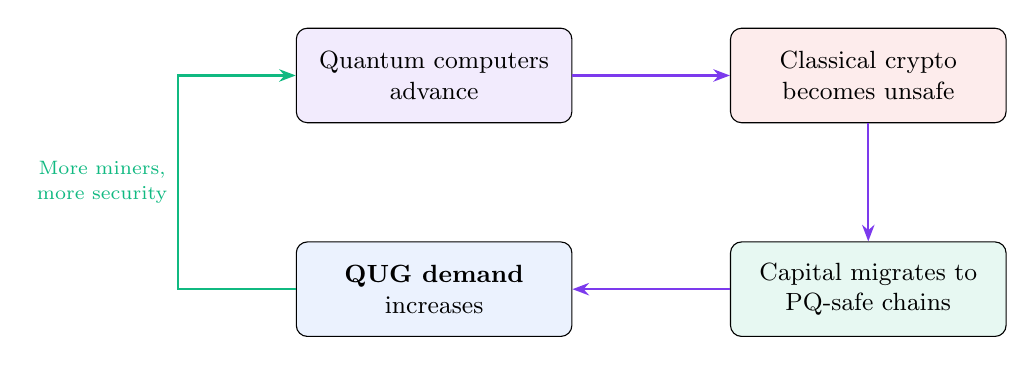
\begin{tikzpicture}[
    node distance=2.5cm,
    every node/.style={align=center, font=\small},
    arrow/.style={-{Stealth[length=6pt]}, thick, qnkpurple}
]
    \node[draw, rounded corners, fill=qnkpurple!10, minimum width=3.5cm, minimum height=1.2cm] (quantum) {Quantum computers\\advance};
    \node[draw, rounded corners, fill=qnkred!10, minimum width=3.5cm, minimum height=1.2cm, right=2cm of quantum] (threat) {Classical crypto\\becomes unsafe};
    \node[draw, rounded corners, fill=qnkgreen!10, minimum width=3.5cm, minimum height=1.2cm, below=1.5cm of threat] (migrate) {Capital migrates to\\PQ-safe chains};
    \node[draw, rounded corners, fill=qnkblue!10, minimum width=3.5cm, minimum height=1.2cm, below=1.5cm of quantum] (qnk) {\textbf{QUG demand}\\increases};

    \draw[arrow] (quantum) -- (threat);
    \draw[arrow] (threat) -- (migrate);
    \draw[arrow] (migrate) -- (qnk);
    \draw[arrow, qnkgreen] (qnk.west) -- +(-1.5,0) |- node[left, pos=0.25] {\scriptsize More miners,\\[-2pt]\scriptsize more security} (quantum.west);
\end{tikzpicture}
\end{center}

\textbf{The mechanism:} Every advance in quantum computing hardware---every IBM, Google, or Chinese government announcement---increases the urgency of post-quantum migration. Q-NarwhalKnight is the \textit{only} production-ready destination. This creates a one-way valve: as quantum progress accelerates (which it inevitably will, given \$30B+ in global quantum investment), capital must flow toward quantum-safe infrastructure. There is no scenario where quantum computing regresses.

\textbf{Mathematical certainty:} Let $P_{\text{quantum}}(t)$ be the probability that quantum computers can break ECDSA by year $t$. This function is \textit{monotonically non-decreasing}: $P_{\text{quantum}}(t_2) \geq P_{\text{quantum}}(t_1)$ for $t_2 > t_1$. The threat can only grow. Migration demand can only increase.

\subsection{Feedback Loop 2: The Regulatory Ratchet}

Government mandates for post-quantum security are \textbf{irreversible}:

\begin{itemize}[leftmargin=1.5em]
    \item \textbf{NIST FIPS 203/204/205 (2024):} Standardized PQ algorithms---cannot be un-standardized
    \item \textbf{NSA CNSA 2.0 (2022):} Mandates PQ for classified systems by 2035---deadline only moves closer
    \item \textbf{EU Cyber Resilience Act (2024):} Requires ``state of the art'' cryptography---PQ is now state of the art
    \item \textbf{DORA (EU, 2025):} Financial institutions must ensure ICT resilience---including crypto-agility
\end{itemize}

Each new regulation \textit{permanently} increases the addressable market for quantum-safe blockchain. Regulations are never repealed to weaken security. This is a ratchet that only tightens.

\subsection{Feedback Loop 3: The Network Effect Flywheel}

\begin{center}
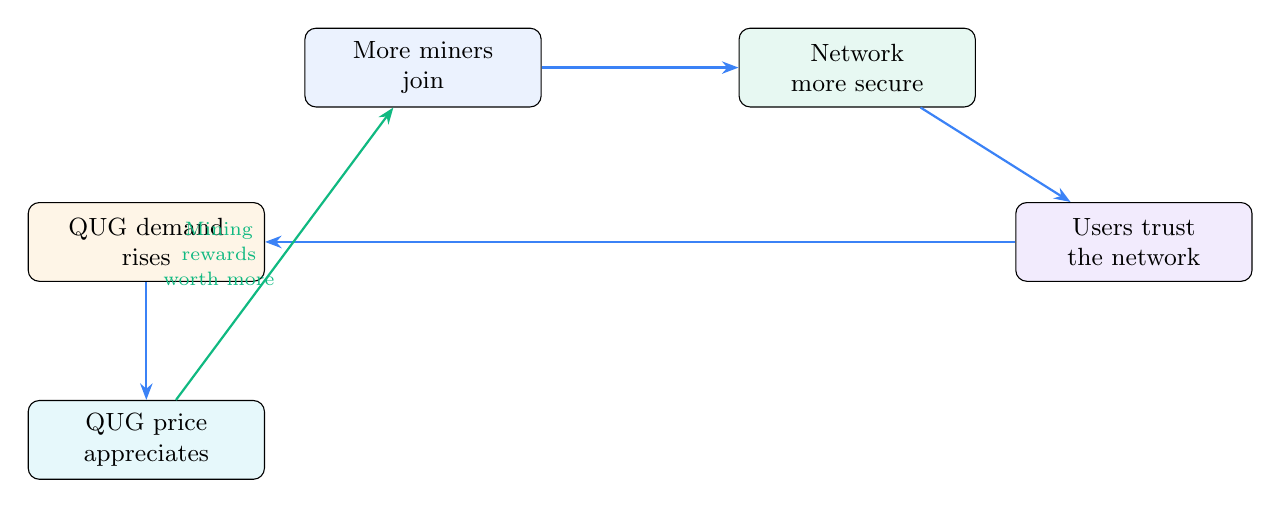
\begin{tikzpicture}[
    node distance=2cm,
    every node/.style={align=center, font=\small},
    arrow/.style={-{Stealth[length=6pt]}, thick, qnkblue}
]
    \node[draw, rounded corners, fill=qnkblue!10, minimum width=3cm, minimum height=1cm] (miners) {More miners\\join};
    \node[draw, rounded corners, fill=qnkgreen!10, minimum width=3cm, minimum height=1cm, right=2.5cm of miners] (security) {Network\\more secure};
    \node[draw, rounded corners, fill=qnkpurple!10, minimum width=3cm, minimum height=1cm, below right=1.2cm and 0.5cm of security] (trust) {Users trust\\the network};
    \node[draw, rounded corners, fill=qnkamber!10, minimum width=3cm, minimum height=1cm, below left=1.2cm and 0.5cm of miners] (demand) {QUG demand\\rises};
    \node[draw, rounded corners, fill=qnkcyan!10, minimum width=3cm, minimum height=1cm, below=1.5cm of demand] (price) {QUG price\\appreciates};

    \draw[arrow] (miners) -- (security);
    \draw[arrow] (security) -- (trust);
    \draw[arrow] (trust) -- (demand);
    \draw[arrow] (demand) -- (price);
    \draw[arrow, qnkgreen] (price) -- node[left] {\scriptsize Mining\\[-2pt]\scriptsize rewards\\[-2pt]\scriptsize worth more} (miners);
\end{tikzpicture}
\end{center}

\subsection{Feedback Loop 4: The Deflationary Supply Schedule}

QUG follows Bitcoin's proven scarcity model with an improvement:

\begin{center}
\begin{tabular}{@{}cccc@{}}
\toprule
\textbf{Period} & \textbf{Block Reward} & \textbf{Annual Emission} & \textbf{Cumulative Supply} \\
\midrule
Year 1 (2026) & 0.001 QUG & $\sim$525,600 QUG & $\sim$525,600 \\
Year 2 (2027) & 0.0005 QUG & $\sim$262,800 QUG & $\sim$788,400 \\
Year 3 (2028) & 0.00025 QUG & $\sim$131,400 QUG & $\sim$919,800 \\
Year 4 (2029) & 0.000125 QUG & $\sim$65,700 QUG & $\sim$985,500 \\
\ldots & $\to 0$ & $\to 0$ & $\to$ 21,000,000 \\
\bottomrule
\end{tabular}
\end{center}

\textbf{Time-based halvings} (annual calendar dates, not block heights) mean that protocol performance improvements \textit{never} accelerate the emission schedule. Faster blocks = more utility, same scarcity.

Combined with increasing demand (Loops 1--3) and fixed/decreasing supply, the price dynamics are structurally asymmetric: \textbf{demand drivers are unbounded while supply is hard-capped}.

\subsection{Feedback Loop 5: The DeFi Gravity Well}

Every DeFi product on Q-NarwhalKnight requires QUG:

\begin{itemize}[leftmargin=1.5em]
    \item \textbf{DEX trading} requires QUG for gas and liquidity pools
    \item \textbf{Quillon Bank} requires QUG collateral for QNKUSD minting
    \item \textbf{Governance voting} requires QUG staking
    \item \textbf{Token deployment} costs QUG
    \item \textbf{NITRO boosts} lock QUG for marketing campaigns
    \item \textbf{AI inference} consumes QUG for computation credits
    \item \textbf{Mining} requires QUG investment in hardware
\end{itemize}

Each product creates a \textbf{QUG sink}---locking tokens in productive use, reducing circulating supply, and increasing scarcity. More products $\to$ more sinks $\to$ less liquid supply $\to$ higher price $\to$ more builders attracted $\to$ more products. This is the DeFi gravity well: once critical mass is achieved, the system pulls in more value with increasing force.

\subsection{Feedback Loop 6: The Technological Moat Compounds Over Time}

\begin{keyinsight}[The 500,000-Line Head Start]
Q-NarwhalKnight's codebase represents an estimated \textbf{25+ engineer-years} of development effort. This is not a whitepaper project with promises---it is 500,000 lines of compiled, tested, deployed Rust code across 83 crates with 4,000+ automated tests.

Any competitor starting today faces:
\begin{itemize}[leftmargin=1.5em]
    \item \textbf{2--3 years} to replicate the post-quantum crypto stack
    \item \textbf{1--2 years} to build the privacy layer (ring sigs + STARKs + Tor)
    \item \textbf{1--2 years} to implement distributed AI inference
    \item \textbf{1 year} to build the DeFi ecosystem
    \item \textbf{Meanwhile}, Q-NarwhalKnight continues advancing
\end{itemize}

The moat is not static---it \textbf{widens} every day as development continues.
\end{keyinsight}

\subsection{The Convergence: Why Failure Requires Active Destruction}

Consider what would need to happen for QUG to \textit{not} appreciate over the medium term:

\begin{enumerate}[leftmargin=1.5em]
    \item Quantum computing would need to \textit{stop advancing entirely} (contradicting \$30B+ investment)
    \item NIST, NSA, and EU would need to \textit{revoke} post-quantum standards (unprecedented)
    \item Privacy demand would need to \textit{decrease} (contradicting every regulatory trend)
    \item Decentralized AI demand would need to \textit{disappear} (contradicting the AI megatrend)
    \item A competitor would need to \textit{replicate} 500K LOC of quantum-safe code faster than we advance (implausible)
    \item Bitcoin's \textit{proven} deflationary scarcity model would need to fail (it has appreciated \$0 $\to$ \$100K+ over 15 years)
\end{enumerate}

\begin{successbox}[The Conclusion]
\textbf{Every secular trend in technology, regulation, and finance converges on Q-NarwhalKnight's value proposition.} The quantum threat grows. Privacy regulation tightens. AI decentralization accelerates. Supply is fixed and halving. The network effect compounds.

This is not a bet on one variable---it is a bet on the continued direction of physics, mathematics, regulatory policy, and computer science. All of these trends would need to \textit{simultaneously reverse} for QUG not to capture significant value. That is not a realistic scenario.
\end{successbox}


% ══════════════════════════════════════════════════════════════
% SECTION 5: ARCHITECTURE
% ══════════════════════════════════════════════════════════════
\section{System Architecture}

\begin{center}
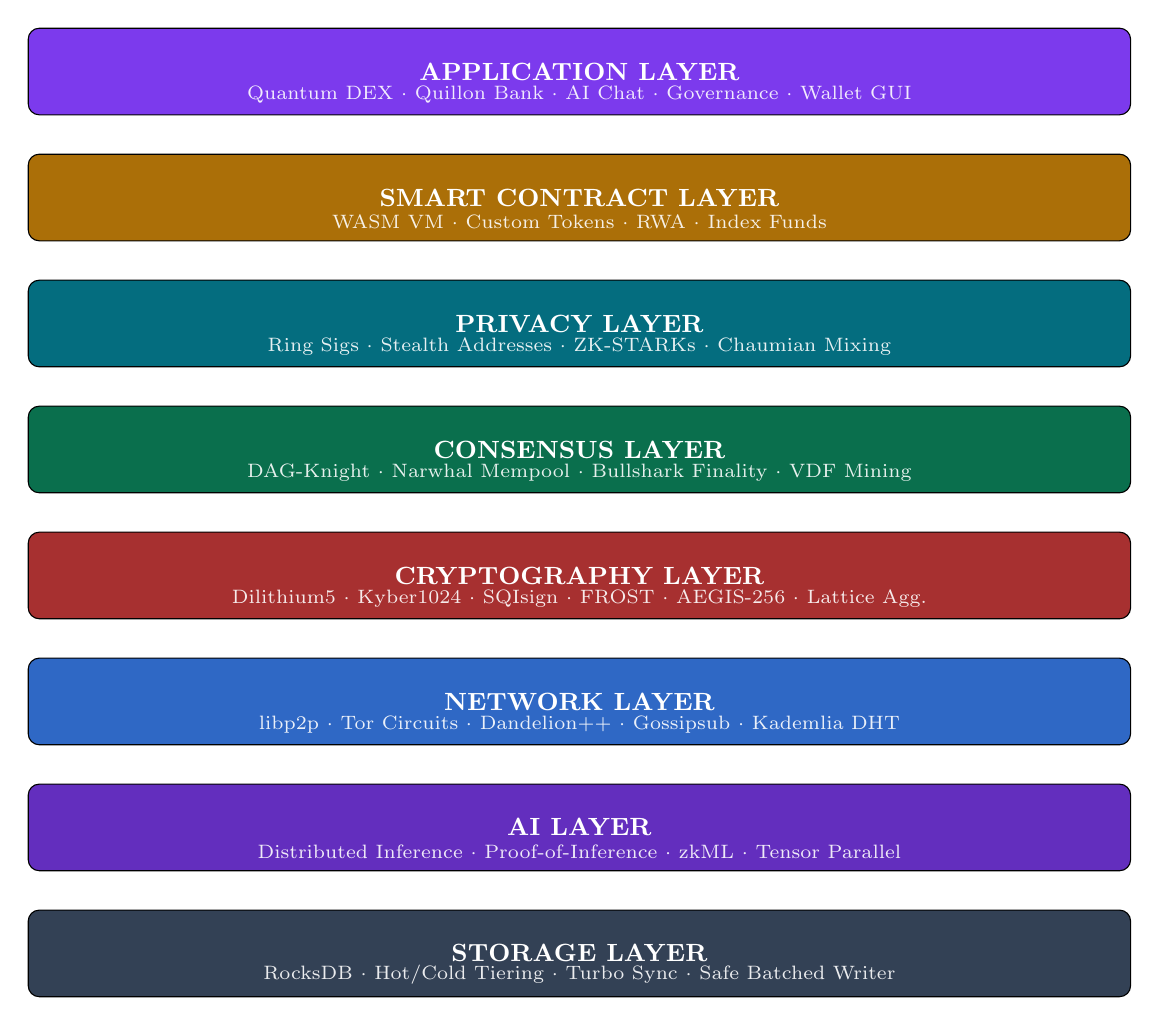
\begin{tikzpicture}[
    layer/.style={draw, rounded corners=4pt, minimum width=14cm, minimum height=1.1cm, font=\small\bfseries, text=white},
    sublabel/.style={font=\scriptsize, text=white, opacity=0.9}
]
    % Layers from bottom to top
    \node[layer, fill=qnkslate] (storage) at (0,0) {STORAGE LAYER};
    \node[sublabel] at (storage.south) [above=1pt] {RocksDB $\cdot$ Hot/Cold Tiering $\cdot$ Turbo Sync $\cdot$ Safe Batched Writer};

    \node[layer, fill=qnkpurple!80!black] (ai) at (0,1.6) {AI LAYER};
    \node[sublabel] at (ai.south) [above=1pt] {Distributed Inference $\cdot$ Proof-of-Inference $\cdot$ zkML $\cdot$ Tensor Parallel};

    \node[layer, fill=qnkblue!80!black] (network) at (0,3.2) {NETWORK LAYER};
    \node[sublabel] at (network.south) [above=1pt] {libp2p $\cdot$ Tor Circuits $\cdot$ Dandelion++ $\cdot$ Gossipsub $\cdot$ Kademlia DHT};

    \node[layer, fill=qnkred!70!black] (crypto) at (0,4.8) {CRYPTOGRAPHY LAYER};
    \node[sublabel] at (crypto.south) [above=1pt] {Dilithium5 $\cdot$ Kyber1024 $\cdot$ SQIsign $\cdot$ FROST $\cdot$ AEGIS-256 $\cdot$ Lattice Agg.};

    \node[layer, fill=qnkgreen!60!black] (consensus) at (0,6.4) {CONSENSUS LAYER};
    \node[sublabel] at (consensus.south) [above=1pt] {DAG-Knight $\cdot$ Narwhal Mempool $\cdot$ Bullshark Finality $\cdot$ VDF Mining};

    \node[layer, fill=qnkcyan!60!black] (privacy) at (0,8.0) {PRIVACY LAYER};
    \node[sublabel] at (privacy.south) [above=1pt] {Ring Sigs $\cdot$ Stealth Addresses $\cdot$ ZK-STARKs $\cdot$ Chaumian Mixing};

    \node[layer, fill=qnkamber!70!black] (contract) at (0,9.6) {SMART CONTRACT LAYER};
    \node[sublabel] at (contract.south) [above=1pt] {WASM VM $\cdot$ Custom Tokens $\cdot$ RWA $\cdot$ Index Funds};

    \node[layer, fill=qnkpurple] (app) at (0,11.2) {APPLICATION LAYER};
    \node[sublabel] at (app.south) [above=1pt] {Quantum DEX $\cdot$ Quillon Bank $\cdot$ AI Chat $\cdot$ Governance $\cdot$ Wallet GUI};
\end{tikzpicture}
\end{center}


% ══════════════════════════════════════════════════════════════
% SECTION 6: TOKENOMICS
% ══════════════════════════════════════════════════════════════
\section{Tokenomics: QUG}

\subsection{Supply Parameters}

\begin{center}
\begin{tabular}{@{}ll@{}}
\toprule
\textbf{Parameter} & \textbf{Value} \\
\midrule
Total Supply (Hard Cap) & 21,000,000 QUG \\
Base Block Reward & 0.001 QUG \\
Halving Schedule & Time-based (annual calendar dates) \\
First Halving & October 26, 2026 \\
Mining Type & SHA-3 + VDF (consumer hardware, ASIC-resistant) \\
Development Fee & 0.5\% of mining rewards \\
Governance Weight & $\text{Power} = \text{Stake} \times (1 + \log_2(\text{Hashes}) / 100)$ \\
\bottomrule
\end{tabular}
\end{center}

\subsection{Why Time-Based Halvings Are Superior}

Traditional blockchains (Bitcoin, Litecoin) couple emission to block height. This creates a dangerous feedback loop: protocol performance improvements that produce faster blocks \textit{accelerate} the halving schedule, making tokenomics unpredictable.

Q-NarwhalKnight's \textbf{time-based halvings} decouple performance from economics. Halvings occur on fixed calendar dates regardless of block production rate. This allows aggressive protocol optimization without unintended economic consequences.

\subsection{Utility Sinks}

QUG is not merely a speculative asset---it is consumed by every network operation:

\begin{multicols}{2}
\begin{itemize}[leftmargin=1.5em]
    \item Transaction gas fees
    \item DEX trading fees
    \item Token deployment costs
    \item Quillon Bank collateral
    \item Governance staking
    \item NITRO boost locks
    \item AI inference credits
    \item Mixing pool participation
\end{itemize}
\end{multicols}


% ══════════════════════════════════════════════════════════════
% SECTION 7: COMPETITIVE LANDSCAPE
% ══════════════════════════════════════════════════════════════
\section{Competitive Landscape}

\begin{center}
\small
\begin{tabular}{@{}p{2.8cm}p{2.5cm}p{1.8cm}p{1.8cm}p{1.8cm}p{1.8cm}@{}}
\toprule
\textbf{Feature} & \textbf{Q-NarwhalKnight} & \textbf{Bitcoin} & \textbf{Ethereum} & \textbf{Solana} & \textbf{Monero} \\
\midrule
Post-Quantum & \textcolor{qnkgreen}{\textbf{Native}} & \textcolor{qnkred}{None} & \textcolor{qnkred}{None} & \textcolor{qnkred}{None} & \textcolor{qnkred}{None} \\
Privacy & \textcolor{qnkgreen}{\textbf{Full Stack}} & \textcolor{qnkred}{None} & \textcolor{qnkamber}{Optional} & \textcolor{qnkred}{None} & \textcolor{qnkgreen}{Ring Sigs} \\
AI & \textcolor{qnkgreen}{\textbf{Distributed}} & \textcolor{qnkred}{None} & \textcolor{qnkred}{None} & \textcolor{qnkred}{None} & \textcolor{qnkred}{None} \\
Built-in DEX & \textcolor{qnkgreen}{\textbf{Full AMM}} & \textcolor{qnkred}{None} & \textcolor{qnkamber}{L2 only} & \textcolor{qnkamber}{Separate} & \textcolor{qnkred}{None} \\
Lending & \textcolor{qnkgreen}{\textbf{Quillon Bank}} & \textcolor{qnkred}{None} & \textcolor{qnkamber}{Separate} & \textcolor{qnkamber}{Separate} & \textcolor{qnkred}{None} \\
ASIC Resistant & \textcolor{qnkgreen}{\textbf{VDF (math)}} & \textcolor{qnkred}{No} & N/A (PoS) & N/A (PoS) & \textcolor{qnkgreen}{RandomX} \\
BFT Threshold & \textcolor{qnkgreen}{\textbf{2f+1}} & N/A & 3f+1 & 3f+1 & N/A \\
ZK Proofs & \textcolor{qnkgreen}{\textbf{Native}} & \textcolor{qnkred}{None} & \textcolor{qnkamber}{L2 only} & \textcolor{qnkred}{None} & \textcolor{qnkred}{None} \\
\bottomrule
\end{tabular}
\end{center}

\begin{keyinsight}[The Only Complete Solution]
No existing blockchain offers \textit{all} of: post-quantum crypto + full privacy + decentralized AI + built-in DeFi + ZK proofs + ASIC-resistant mining + improved BFT. Q-NarwhalKnight is not competing in one category---it is the only entry in the intersection of all categories.
\end{keyinsight}


% ══════════════════════════════════════════════════════════════
% SECTION 8: TRACTION
% ══════════════════════════════════════════════════════════════
\section{Traction and Development Status}

\subsection{What Has Been Built}

\begin{center}
\begin{tabular}{@{}p{5cm}p{2cm}p{7cm}@{}}
\toprule
\textbf{Component} & \textbf{Status} & \textbf{Details} \\
\midrule
Core Blockchain & \textcolor{qnkgreen}{Complete} & DAG-Knight consensus, block production, P2P sync \\
Post-Quantum Crypto & \textcolor{qnkgreen}{Complete} & Dilithium5, Kyber1024, SQIsign, FROST, AEGIS \\
Privacy Stack & \textcolor{qnkgreen}{Complete} & Ring sigs, stealth, ZK-STARKs, Tor, Dandelion++ \\
Distributed AI & \textcolor{qnkgreen}{Complete} & Mistral-7B inference across validator nodes \\
DEX \& DeFi & \textcolor{qnkgreen}{Complete} & AMM, stablecoin, lending, index funds \\
Mining System & \textcolor{qnkgreen}{Complete} & VDF + SHA-3, pool support, GPU acceleration \\
Wallet GUI & \textcolor{qnkgreen}{Complete} & Web-based quantum wallet at quillon.xyz \\
Test Suite & \textcolor{qnkgreen}{Complete} & 4,000+ tests with mainnet safety checks \\
Whitepapers & \textcolor{qnkgreen}{Complete} & 50-page physics whitepaper, multiple technical docs \\
Cross-Chain Bridges & \textcolor{qnkamber}{Planned} & Infrastructure exists, activation pending \\
Enterprise SDK & \textcolor{qnkamber}{Planned} & Q1 2027 \\
\bottomrule
\end{tabular}
\end{center}

\subsection{Development Roadmap}

\begin{center}
\begin{tabular}{@{}p{2.5cm}p{11.5cm}@{}}
\toprule
\textbf{Timeline} & \textbf{Milestone} \\
\midrule
\textbf{Q1 2026} & Testnet live with mining, DEX, AI, and P2P sync \\
\textbf{Q2 2026} & Independent security audit (post-quantum cryptography focus) \\
\textbf{Q3 2026} & Mainnet launch candidate; multi-region validator network \\
\textbf{Q4 2026} & \textbf{Mainnet launch + first halving event (October 26)} \\
\textbf{Q1 2027} & Enterprise SDK; sovereign chain toolkit \\
\textbf{Q2 2027} & Cross-chain bridges (Bitcoin, Ethereum); mobile wallet \\
\textbf{Q3 2027} & Hardware wallet integration; institutional custody support \\
\textbf{Q4 2027} & Advanced AI models (vision, multimodal); QRNG hardware partnerships \\
\bottomrule
\end{tabular}
\end{center}


% ══════════════════════════════════════════════════════════════
% SECTION 9: RISK FACTORS
% ══════════════════════════════════════════════════════════════
\section{Risk Factors and Mitigations}

\begin{center}
\begin{tabular}{@{}p{4cm}p{3cm}p{7cm}@{}}
\toprule
\textbf{Risk} & \textbf{Likelihood} & \textbf{Mitigation} \\
\midrule
PQ algorithm broken & Very Low & Crypto-agile design allows algorithm swap without hard fork \\
Competitor replication & Low & 500K LOC head start; moat widens daily \\
Regulatory adversity & Medium & Privacy is optional/configurable; compliance engine built-in \\
Adoption delay & Medium & Revenue from mining; low burn rate; long runway \\
Quantum timeline slower & Low-Medium & PQ crypto has value even without quantum threat (smaller sigs, etc.) \\
Smart contract bugs & Medium & WASM sandboxing; ZK validity proofs; formal verification planned \\
\bottomrule
\end{tabular}
\end{center}


% ══════════════════════════════════════════════════════════════
% SECTION 10: THE ASK
% ══════════════════════════════════════════════════════════════
\section{Investment Opportunity}

\subsection{Use of Funds}

\begin{center}
\begin{tabular}{@{}p{5cm}p{9cm}@{}}
\toprule
\textbf{Category} & \textbf{Purpose} \\
\midrule
Security Audit (30\%) & Independent verification of PQ crypto; formal methods analysis \\
Infrastructure (25\%) & Multi-region validator deployment; testnet scaling \\
Enterprise BD (20\%) & Sovereign state pilots; financial institution partnerships \\
Ecosystem (15\%) & Developer tools, SDKs, documentation, hackathons \\
Operations (10\%) & Legal, compliance, administrative \\
\bottomrule
\end{tabular}
\end{center}

\subsection{Why Invest Now}

\begin{enumerate}[leftmargin=1.5em]
    \item \textbf{First-mover advantage}: No other L1 has native PQ crypto + privacy + AI. Period.
    \item \textbf{Regulatory tailwind}: NIST/NSA/EU mandating quantum-safe transition creates guaranteed demand.
    \item \textbf{Technical moat}: 500K LOC, 83 crates, 4K+ tests---\textit{years} of head start.
    \item \textbf{Physics-grounded}: Not ad-hoc engineering---mathematically proven consensus with a 50-page whitepaper.
    \item \textbf{Complete stack}: Not just a chain---DEX, bank, AI, privacy, governance, all production-ready.
    \item \textbf{Fair launch}: VDF mining (no premine advantage), time-based halvings, 0.5\% dev fee only.
    \item \textbf{Pre-mainnet entry}: Early investors enter before mainnet launch and first halving (Q4 2026).
\end{enumerate}

\vspace{1cm}

\begin{center}
\begin{tcolorbox}[
    enhanced,
    colback=qnkpurple!8,
    colframe=qnkpurple,
    boxrule=1.5pt,
    arc=8pt,
    width=14cm,
    shadow={2mm}{-2mm}{0mm}{black!20}
]
\begin{center}
{\Large\bfseries\textcolor{qnkpurple}{The quantum computing threat to blockchain isn't coming---it's here.}}

\vspace{0.5cm}

{\large\textcolor{qnkslate}{Q-NarwhalKnight is the answer.}}

\vspace{0.5cm}

{\small\textcolor{qnkslate}{
\textit{``Physical laws should have mathematical beauty.''} --- Paul Dirac\\[6pt]
Q-NarwhalKnight's consensus dynamics satisfy this criterion.
}}
\end{center}
\end{tcolorbox}
\end{center}

\vfill

\begin{center}
\textcolor{qnkslate}{\rule{8cm}{0.5pt}}

\vspace{0.3cm}

{\small
\textbf{Website:} \url{https://quillon.xyz} \quad$\cdot$\quad \textbf{Live Testnet:} \url{https://quillon.xyz}

\vspace{0.2cm}

\textbf{Whitepaper:} \textit{``Quantum Physics in Q-NarwhalKnight: A Comprehensive Analysis of Quantum-Enhanced Distributed Consensus Systems with String-Theoretic Resonance''} (v3.0, 50 pages)
}
\end{center}

% ══════════════════════════════════════════════════════════════
% LEGAL DISCLAIMER
% ══════════════════════════════════════════════════════════════
\vspace{1cm}
\begin{center}
\begin{minipage}{13cm}
{\scriptsize\textcolor{gray}{
\textbf{Disclaimer:} This document is for informational purposes only and does not constitute an offer or solicitation to buy or sell any securities or tokens. Past performance is not indicative of future results. Cryptocurrency investments carry significant risk, including the potential loss of all invested capital. The ``self-reinforcing dynamics'' described herein are theoretical mechanisms based on economic and game-theoretic analysis; actual outcomes depend on market conditions, adoption rates, regulatory developments, and technological factors beyond the control of any individual party. Prospective investors should conduct their own due diligence and consult qualified financial and legal advisors. The statements about quantum computing timelines reflect current scientific consensus and publicly available research; actual quantum computing progress may differ materially from projections. This document contains forward-looking statements that involve risks and uncertainties.
}}
\end{minipage}
\end{center}

\end{document}
